\section{Analysis of results}
Benchmarks results have been obtained for all application and available processors combinations to be able to observe the real behaviour of the selected applications.
Each test has been repeated twice with the measurements for minimum wall time selected to be reported. This section presents the most interesting findings and conclusions from these tests.%% are presented in Section~\ref{sec:}.

The group of benchmarked social simulation software covers applications for pre-processing and simulation of agent-based models. Two typical pre-processing tasks have been considered: converting shape files to rasters and producing synthetic populations. The benchmarks have shown that conversion from shape files to rasters is very demanding in terms of RAM while I/O and CPU requirements are rather low. In order to study computational requirements to applications that generate synthetic populations, a simple parallel version of the celebrated iterative proportional fitting (IPF) method was implemented. This implementation heavily uses dense linear algebra kernels provided by a highly optimised ScaLAPACK library. The benchmarks demonstrate high performance of IPF on different architectures. Neither RAM, nor I/O of modern architectures are limiting factors for IPF performance. Along with ABMS pre-processing applications, a simple agent-based model of diffusion with the help of distributed ABMS frameworks following two different parallelization strategies for ABMs with raster inputs was benchmarked. The first framework (Pandora) written in C++ parallelises the simulation process via splitting of rasters on even pieces and distributing them between MPI processes, while the second framework (ABM4py) is a Python code, which implements the graph-based parallelization approach. Despite strong difference in parallelization strategies, in both cases, the observation delivered the same pattern: ABMS applications produce a big amount of output which has a strong negative impact on application performance. As a consequence, according to the "toy" ABMs, being I/O bound, current ABMS frameworks for HPC have moderate requirements to CPU performance. Nevertheless, it must be emphasised that the results can look differently for complex models with sophisticated agent activities and models which can be reduced to iterations with sparse-matrix dense-vector operations, thus, the benchmarks for ABMS frameworks are not very illuminative and must be extended with more sophisticated models to draw stronger conclusions. But discussion of the new ABMS models for benchmarking goes beyond the scope of this text. Table~\ref{tab:bottlenecks_hardware} shortly summarises information about scalability of the benchmarked social simulation software and hardware bottlenecks.

\begin{table}[htbp]
\begin{minipage}[t]{1\textwidth}
\caption{Bottlenecks in the hardware and scalability for the application from social simulation software stack}
\label{tab:bottlenecks_hardware}
\end{minipage}
\begin{tabular}{cl|c|c|c|c|c|}
\cline{3-7}
 &  & \multicolumn{2}{c|}{pre-processing} & \multicolumn{3}{c|}{ABMS (with raster input)} \\ \cline{3-7} 
 &  & \multirow{2}{*}{rastering} & \multirow{2}{*}{IPF} & \multicolumn{2}{c|}{Pandora} & \multicolumn{1}{l|}{ABM4py} \\ \cline{5-7} 
 &  &  &  & \multicolumn{1}{l|}{Europe} & \multicolumn{1}{l|}{World} & \multicolumn{1}{l|}{128x128} \\ \hline
\multicolumn{1}{|c|}{\multirow{4}{*}{Bottlenecks}} & CPU &  & \checkmark &  &  &  \\ \cline{2-7} 
\multicolumn{1}{|c|}{} & RAM &  &  &  &  &  \\ \cline{2-7} 
\multicolumn{1}{|c|}{} & IO &  &  & output & output & output \\ \cline{2-7} 
\multicolumn{1}{|c|}{} & Network & N.A. &  &  &  &  \\ \hline
\multicolumn{2}{|c|}{Scalability \ *} & serial & $\ge$1400 &  $\approx$128 & $\approx$700 & $\approx$128 \\ \hline
\end{tabular}
\newline
\raggedright{* maximum\ number\ of\ utilised\ cores\ for\ Eagle\ cluster}
\end{table}


The group of benchmarked CFD applications includes large scale tools that simulate GSS-related scenarios like natural disasters (hurricanes, earthquakes), spread of air pollution and weather prediction. More specifically, the following open-source CFD codes have been selected the benchmarking purposes: HRWF – a parallel implementation of the hurricane weather research and forecasting (HWRF); OpenSWPC – an integrated parallel simulation code for modelling seismic wave propagation in 3D heterogeneous viscoelastic media; CMAQ – a community multiscale air quality modelling system, which combines CFD codes for conducting large scale air quality model simulations.

As expected, the benchmarks confirm that CFD applications are in general CPU-bound (e.g. Figure~\ref{fig:openswpc_scalability}) in contrast to the social simulation software. At the same, time output makes a solid contribution to the total elapsed time for such applications like CCTM and CM1 (e.g. Figure~\ref{fig:cm1_arm}) which, in turn, imposed additional performance constraints on architectures with poor I/O speed. Nevertheless, it was observed that at some architectures memory was also a bottleneck for some choices of the number of MPI processes. In addition, it was noticed that OpenSWPC is memory bound for the small number of MPI processes. The relevant information about scalability of the benchmarked CFD applications and hardware bottlenecks is outlined it Table~\ref{tab:bottlenecks_cfd_hardware}

\begin{table}[htbp]
\begin{minipage}[t]{1\textwidth}
\caption{Bottlenecks in the hardware and scalability for the large-scale CFD applications}
\label{tab:bottlenecks_cfd_hardware}
\end{minipage}
\begin{tabular}{cl|c|c|c|c|}
\cline{3-6}
 &  & HWRF & OpenSWPC & CMAQ/CCTM) & \multicolumn{1}{l|}{CM1} \\ \hline
\multicolumn{1}{|c|}{\multirow{4}{*}{Bottlenecks}} & CPU & \checkmark & \checkmark & \checkmark & \checkmark \\ \cline{2-6} 
\multicolumn{1}{|c|}{} & RAM &  & \checkmark &  &  \\ \cline{2-6} 
\multicolumn{1}{|c|}{} & IO & input &  & output & output \\ \cline{2-6} 
\multicolumn{1}{|c|}{} & Network &  &  &  &  \\ \hline
\multicolumn{2}{|c|}{Scalability *} & $\ge$128 & $\ge$128 & $\ge$128 & $\ge$128 \\ \hline
\end{tabular}
\newline
\raggedright{* maximum\ number\ of\ utilized\ cores\ for\ Eagle\ cluster}
\end{table}

As Tables ~\ref{tab:bottlenecks_hardware} and~\ref{tab:bottlenecks_cfd_hardware} illustrate, most of the distributed GSS applications are memory bound. Even large-scale CFD codes can be bound by I/O and RAM under special circumstances. It allows to formulate the conclusion that the fast memory is an essential requirement to HPC clusters for GSS applications whereas high CPU’s clock frequency plays a less important role. Moreover, since many state-of-the-art GSS applications deal with large input and output files, it is believed that GSS software developers should invest more time into designing file-avoiding applications. The scalability tests show that hyperthreading provides little performance improvements for most of the GSS applications. Therefore, it makes little sense to invest money in expensive massively multithreaded chips (like Power8) for GSS users. It is also recommended to avoid clusters with GPU accelerated nodes since only few popular GSS applications benefit from GPUs. In particular, among widely used general-purpose ABMS frameworks and problem-specific ABMS codes for HPCs, only the FLAME-GPU (Flexible Larg-scale Agent Modelling Environment) \cite{2011:flame_gpu} \cite{2018:flame_gpu} framework utilises GPUs. Weak use of GPUs is also partially related to the fact that most social science applications are memory bound. Being more specific, among the architectures used in benchmarking, we recommend to build clusters upon ARM Hi1616 if energy efficiency is a crucial requirement, or upon Intel\textregistered Xeon\textregistered Gold 6140 if performance is a first priority while relatively high operating expense and capital expenditure are not an issue.

\begin{figure*}
\centering
%% 1 row - OpenSWPC
    \begin{subfigure}[t]{0.48\textwidth}
        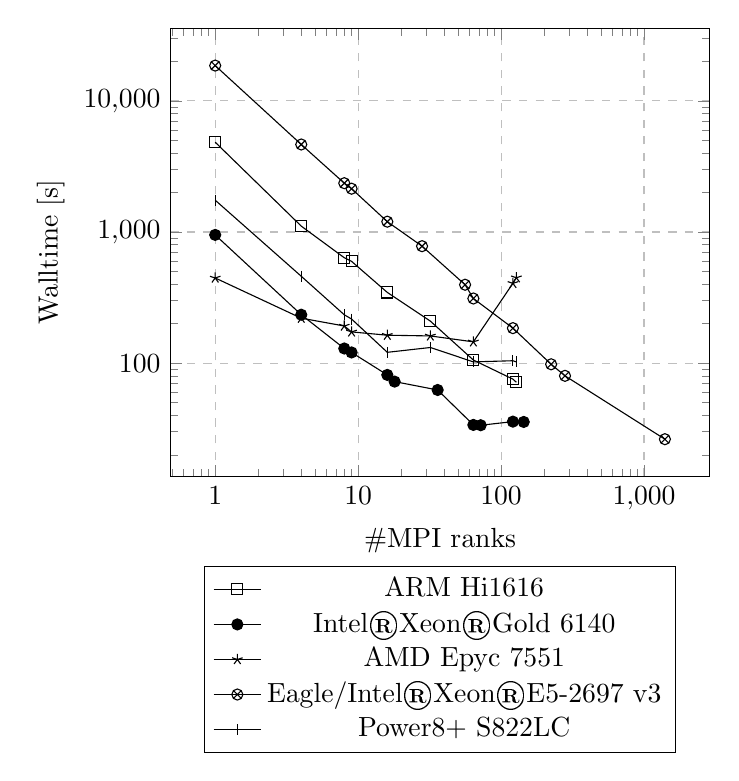
\begin{tikzpicture}[scale=1, baseline]
            \begin{axis}[
            %width=1.3\textwidth,
            xmode=log,
            ymode=log,
            log ticks with fixed point,
            scaled y ticks=real:1e3
            axis lines = left,
            xlabel = \#MPI ranks,
            ylabel = {Walltime [s]},
            legend style={at={(0.5,-0.2)},
            	    anchor=north,legend columns=1},
            xmajorgrids=true,
            ymajorgrids=true,
            grid style=dashed,
            ]
                %ARM
                \addplot [
                    domain=1:150, 
                    color=black,
                    mark=square,
                    ]
                    coordinates {
                   (1,4840)(4,1109)(8,636.4)(9,596.9)(16,346.1)(32,209.1)(64,105.6)(121,75.5)(128,71.4)
                    };
                \addlegendentry{ARM Hi1616}
                %Intel 6140
                \addplot [
                    domain=1:150, 
                    color=black,
                    mark=*,
                ]
                coordinates {
                    (1,950.4)(4,234)(8,129.3)(9,120.6)(16,81.3)(18,72.3)(36,62.4)(64,33.8)(72,33.6)(121,35.8)(144,35.6)
                    };
                \addlegendentry{Intel\textregistered Xeon\textregistered Gold 6140}
                %AMD Epyc
                \addplot [
                    domain=1:150, 
                    color=black,
                    mark=star,
                    ]
                    coordinates {
                   (1,446.1)(4,220.2)(8,192)(9,173)(16,163.3)(32,161.21)(64,145.3)(121,406)(128,448.1)
                    };
                \addlegendentry{AMD Epyc 7551}
                %Eagle
                \addplot [
                    domain=1:1400, 
                    color=black,
                    mark=otimes,
                    ]
                    coordinates {                    (1,18584.8)(4,4649.8)(8,2356.4)(9,2139.0)(16,1198.7)(28,779.8)(56,396.2)(64,311.1)(121,184.9)(224,98)(280,80)(38.2)(1400,26.3)
                    };
                \addlegendentry{Eagle/Intel\textregistered Xeon\textregistered E5-2697 v3}
                %Power
                \addplot [
                    domain=1:150, 
                    color=black,
                    mark=|,
                    ]
                    coordinates {
                    (1,1748.7)(4,459.8)(8,233.7)(9,216.9)(16,120.9)(32,131.6)(64,102.2)(121,104.3)(128,102.2)
                    };
                \addlegendentry{Power8+ S822LC}
            \end{axis}
        \end{tikzpicture}
        \caption{OpenSWPC scalability}
        \label{fig:openswpc_scalability}
    \end{subfigure}\hfill
    \begin{subfigure}[t]{0.48\textwidth}
        \centering
        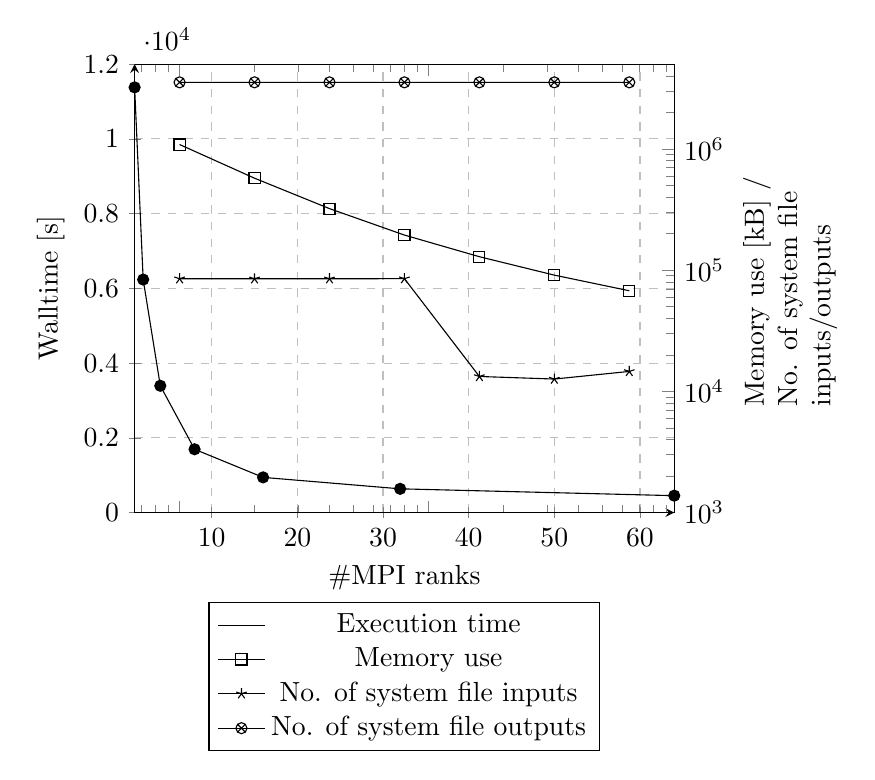
\begin{tikzpicture}[scale=1, baseline]
            \begin{axis}[
            %    width=1\textwidth,
                axis y line*=left,
                axis lines = left,
                xlabel = \#MPI ranks,
                ylabel = {Walltime [s]},
                xmajorgrids=true,
                ymajorgrids=true,
                grid style=dashed,
                ymin=1, ymax=12000,
                ]
                %Execution time
                \addplot [
                    domain=1:70, 
                    color=black,
                    mark=*,
                ]
                coordinates {(1,11379.8)(2,6236)(4,3393.1)(8,1694.1)(16,941.5)(32,635.1)(64,452)};
                \label{openswpc_execution_time}
            \end{axis}
            \begin{axis}[
                xmode=log,
                ymode=log,
                xticklabel=\empty,
                axis y line*=right,
                scaled ticks=false,
                y tick label style={/pgf/number format/.cd,sci,sci e},
                ymin=1000, ymax=5000000,
                ylabel style={text width=3cm},
                ylabel = {Memory use {[kB]} {/} No. of system file inputs/outputs},
                legend style={at={(0.5,-0.2)},
                	    anchor=north,legend columns=1},
                grid style=dashed,
                ]
                \addlegendimage{/pgfplots/refstyle=openswpc_execution_time}
                \addlegendentry{Execution time}
                %RAM
                \addplot [
                    domain=1:70, 
                    color=black,
                    mark=square,
                    ]
                    coordinates {(1,1086860)(2,573320)(4,321660)(8,194592)(16,128996)(32,90904)(64,67560)};
                \addlegendentry{Memory use}
                %#inputs
                \addplot [
                    domain=1:70, 
                    color=black,
                    mark=star,
                    ]
                    coordinates {(1,84891)(2,84808)(4,84876)(8,84992)(16,13256)(32,12624)(64,14592)};
                \addlegendentry{No. of system file inputs}
                %#outputs
                \addplot [
                    color=black,
                    mark=otimes,
                    ]
                    coordinates {(1,3541296)(2,3544032)(4,3543000)(8,3542488)(16,3542144)(32,3542024)(64,3541936)};
                \addlegendentry{No. of system file outputs}
            \end{axis}
            \end{tikzpicture}
          \caption{OpenSWPC results for XXXX}
          \label{fig:openswpc_arm}
      \end{subfigure}\bigbreak
  %%2 row - CMAQ/CCTM
  \begin{subfigure}[t]{0.48\textwidth}
   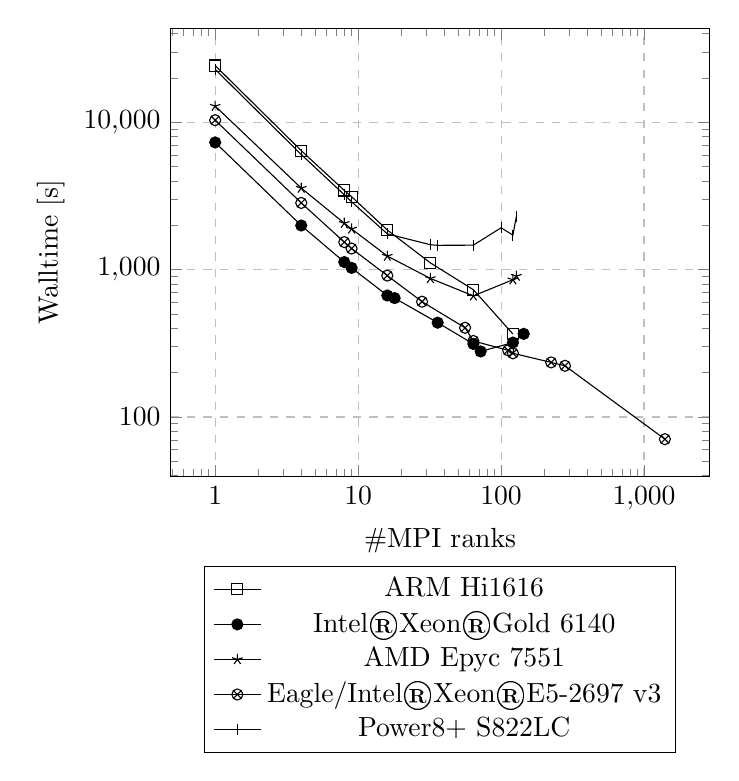
\begin{tikzpicture}[scale=1, baseline]
    \begin{axis}[
    %    width=1.3\textwidth,
        xmode=log,
        ymode=log,
        log ticks with fixed point,
        scaled y ticks=real:1e3
        axis lines = left,
        xlabel = \#MPI ranks,
        ylabel = {Walltime [s]},
        legend style={at={(0.5,-0.2)},
        	    anchor=north,legend columns=1},
        xmajorgrids=true,
        ymajorgrids=true,
        grid style=dashed,
        ]
        %ARM
        \addplot [
            domain=1:150, 
            color=black,
            mark=square,
            ]
            coordinates {
            (1,24239.6)(4,6416.1)(8,3445.6)(9,3124.6)(16,1856.3)(32,1111.4)(64,730.7)(121,365.4)
            };
        \addlegendentry{ARM Hi1616}
        %Intel 6140
        \addplot [
            domain=1:150, 
            color=black,
            mark=*,
        ]
        coordinates {
            (1,7294.6)(4,1991.6)(8,1125.1)(9,1027.3)(16,667.5)(18,640.7)(36,436.4)(64,313.2)(72,278.4)(121,320)(144,366.5)
            };
        \addlegendentry{Intel\textregistered Xeon\textregistered Gold 6140}
        %AMD Epyc
        \addplot [
            domain=1:150, 
            color=black,
            mark=star,
            ]
            coordinates {
            (1,12872.6)(4,3574.8)(8,2064.3)(9,1888.6)(16,1235.9)(32,871.8)(64,663.3)(121,853.9)(128,902.9)
            };
        \addlegendentry{AMD Epyc 7551}
        %Eagle
        \addplot [
            domain=1:1400,
            color=black,
            mark=otimes,
            ]
            coordinates {
            (1,10323.7)(4,2834.3)(8,1537)(9,1389.7)(16,910.7)(28,605.8)(56,402.9)(64,327.9)(112,283.3)(121,270.5)(224,234.6)(280,222.5)(1400,70.7)
            };
        \addlegendentry{Eagle/Intel\textregistered Xeon\textregistered E5-2697 v3}
        %Power
        \addplot [
            domain=1:150, 
            color=black,
            mark=|,
            ]
            coordinates {
            (1,22849.8)(4,6036.1)(8,3220.3)(9,2885.9)(16,1748.2)(32,1476)(36,1461.4)(64,1465.4)(100,1921.8)(121,1714.5)(128,2297.7)
            };
        \addlegendentry{Power8+ S822LC}
        \end{axis}
        \end{tikzpicture}
  \caption{CMAQ/CCTM\ scalability}
  \label{fig:cmaq_scalability}
 \end{subfigure}\hfill
 \begin{subfigure}[t]{0.48\textwidth}
  \centering
        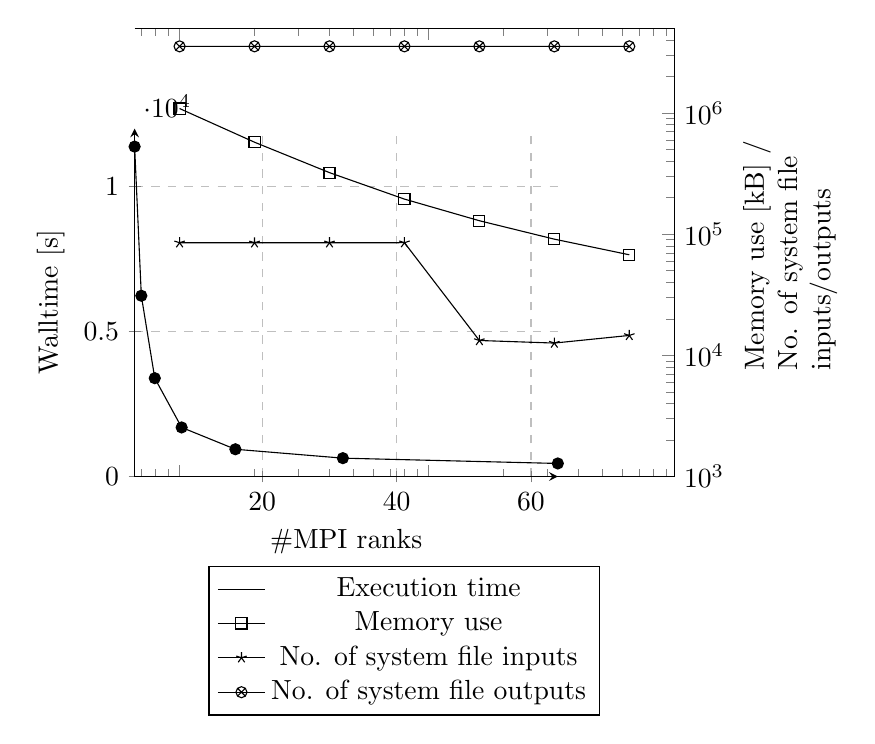
\begin{tikzpicture}[scale=1, baseline]
        \begin{axis}[
            height=6cm,
            axis y line*=left,
            axis lines = left,
            xlabel = \#MPI ranks,
            ylabel = {Walltime [s]},
            xmajorgrids=true,
            ymajorgrids=true,
            grid style=dashed,
            ymin=1, ymax=12000,
            ]
            %Execution time
            \addplot [
                domain=1:70, 
                color=black,
                mark=*,
            ]
            coordinates {(1,11379.8)(2,6236)(4,3393.1)(8,1694.1)(16,941.5)(32,635.1)(64,452)};
            \label{cmaq_execution_time}
            \end{axis}
            \begin{axis}[
                xmode=log,
                ymode=log,
                xticklabel=\empty,
                axis y line*=right,
                scaled ticks=false,
                y tick label style={/pgf/number format/.cd,sci,sci e},
                ymin=1000, ymax=5000000,
                ylabel style={text width=3cm},
                ylabel = {Memory use {[kB]} {/} No. of system file inputs/outputs
            },
                legend style={at={(0.5,-0.2)},
                	    anchor=north,legend columns=1},
                grid style=dashed,
                ]
            \addlegendimage{/pgfplots/refstyle=cmaq_execution_time}\addlegendentry{Execution time}
            %RAM
            \addplot [
                domain=1:70, 
                color=black,
                mark=square,
                ]
                coordinates {(1,1086860)(2,573320)(4,321660)(8,194592)(16,128996)(32,90904)(64,67560)};
            \addlegendentry{Memory use}
            %#inputs
            \addplot [
                domain=1:70, 
                color=black,
                mark=star,
                ]
                coordinates {(1,84891)(2,84808)(4,84876)(8,84992)(16,13256)(32,12624)(64,14592)};
            \addlegendentry{No. of system file inputs}
            %#outputs
            \addplot [
                color=black,
                mark=otimes,
                ]
                coordinates {(1,3541296)(2,3544032)(4,3543000)(8,3542488)(16,3542144)(32,3542024)(64,3541936)};
            \addlegendentry{No. of system file outputs}
            \end{axis}
            \end{tikzpicture}
    \caption{CCTM results for XXXX}
    \label{fig:cctm_arm}
    \end{subfigure}\hfill
%%3 row - CM1
    \begin{subfigure}[t]{0.48\textwidth}
        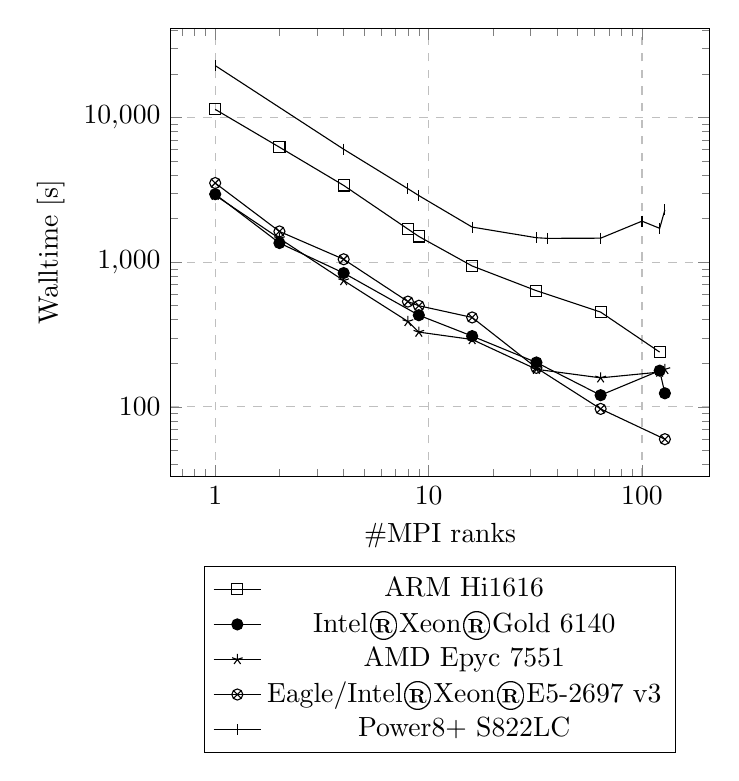
\begin{tikzpicture}[scale=1, baseline]
        \begin{axis}[
            xmode=log,
            ymode=log,
            log ticks with fixed point,
            scaled y ticks=real:1e3
            axis lines = left,
            xlabel = \#MPI ranks,
            ylabel = {Walltime [s]},
            legend style={at={(0.5,-0.2)},
            	    anchor=north,legend columns=1},
            xmajorgrids=true,
            ymajorgrids=true,
            grid style=dashed,
            ]
            %ARM
            \addplot [
                domain=1:150, 
                color=black,
                mark=square,
                ]
                coordinates {
                (1,11379.8)(2,6236)(4,3393.1)(8,1694.1)(9,1505.9)(16,941.5)(32,635.1)(64,452)(121,239.1)
                };
            \addlegendentry{ARM Hi1616}
            %Intel 6140
            \addplot [
                domain=1:150, 
                color=black,
                mark=*,
            ]
            coordinates {
                (1,2952)(2,1356.7)(4,841.2)(9,430)(16,308.4)(32,202.7)(64,120.4)(121,178)(128,124.1)
                };
            \addlegendentry{Intel\textregistered Xeon\textregistered Gold 6140}
            %AMD Epyc
            \addplot [
                domain=1:150, 
                color=black,
                mark=star,
                ]
                coordinates {
                (1,2900)(2,1459)(4,746.8)(8,389.4)(9,328.7)(16,292.2)(32,181.9)(64,158.7)(121,174)(128,181.5)
                };
            \addlegendentry{AMD Epyc 7551}
            %Eagle
            \addplot [
                domain=1:1400,
                color=black,
                mark=otimes,
                ]
                coordinates {
                (1,3524)(2,1631.4)(4,1047.2)(8,534)(9,500)(16,415)(32,186.1)(64,96.8)(128,59.8)
                };
            \addlegendentry{Eagle/Intel\textregistered Xeon\textregistered E5-2697 v3}
            %Power
            \addplot [
                domain=1:150, 
                color=black,
                mark=|,
                ]
                coordinates {
                (1,22849.8)(4,6036.1)(8,3220.3)(9,2885.9)(16,1748.2)(32,1476)(36,1461.4)(64,1465.4)(100,1921.8)(121,1714.5)(128,2297.7)
                };
            \addlegendentry{Power8+ S822LC}
            \end{axis}
            \end{tikzpicture}
        \caption{CM1\ scalability}
        \label{fig:cm1_scalability}
    \end{subfigure}\hfill
    \begin{subfigure}[t]{0.48\textwidth}
    \centering
        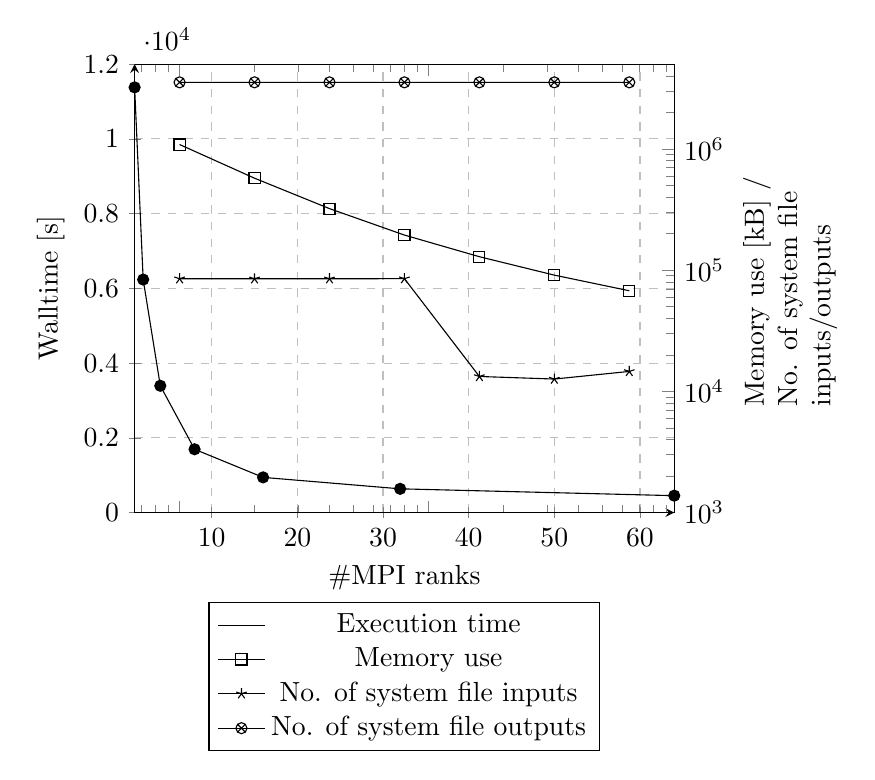
\begin{tikzpicture}[scale=1, baseline]
        \begin{axis}[
        %    width=1\textwidth,
            axis y line*=left,
            axis lines = left,
            xlabel = \#MPI ranks,
            ylabel = {Walltime [s]},
            xmajorgrids=true,
            ymajorgrids=true,
            grid style=dashed,
            ymin=1, ymax=12000,
            ]
            %Execution time
            \addplot [
                domain=1:70, 
                color=black,
                mark=*,
            ]
            coordinates {(1,11379.8)(2,6236)(4,3393.1)(8,1694.1)(16,941.5)(32,635.1)(64,452)};
            \label{cm1_execution_time}
            \end{axis}
            \begin{axis}[
            xmode=log,
            ymode=log,
            xticklabel=\empty,
            axis y line*=right,
            scaled ticks=false,
            y tick label style={/pgf/number format/.cd,sci,sci e},
            ymin=1000, ymax=5000000,
            ylabel style={text width=3cm},
            ylabel = {Memory use {[kB]} {/} No. of system file inputs/outputs
        },
            legend style={at={(0.5,-0.2)},
            	    anchor=north,legend columns=1},
            grid style=dashed,
            ]
            \addlegendimage{/pgfplots/refstyle=cm1_execution_time}\addlegendentry{Execution time}
            %RAM
            \addplot [
                domain=1:70, 
                color=black,
                mark=square,
                ]
                coordinates {(1,1086860)(2,573320)(4,321660)(8,194592)(16,128996)(32,90904)(64,67560)};
            \addlegendentry{Memory use}
            %#inputs
            \addplot [
                domain=1:70, 
                color=black,
                mark=star,
                ]
                coordinates {(1,84891)(2,84808)(4,84876)(8,84992)(16,13256)(32,12624)(64,14592)};
            \addlegendentry{No. of system file inputs}
            %#outputs
            \addplot [
                color=black,
                mark=otimes,
                ]
                coordinates {(1,3541296)(2,3544032)(4,3543000)(8,3542488)(16,3542144)(32,3542024)(64,3541936)};
            \addlegendentry{No. of system file outputs}
            \end{axis}
            \end{tikzpicture}
  \caption{CM1 results for ARM Hi616}
  \label{fig:cm1_arm}
  \end{subfigure}%
  \bigbreak
  \caption{Detailed benchmarking results for CFD applications}
\end{figure*}